\documentclass[tikz]{standalone}
\usepackage{pgfplots}
\usepackage{times}
\usepackage[scaled=.9]{helvet}
%\renewcommand{\familydefault}{\sfdefault}
\pgfplotsset{compat=1.18}

\begin{document}

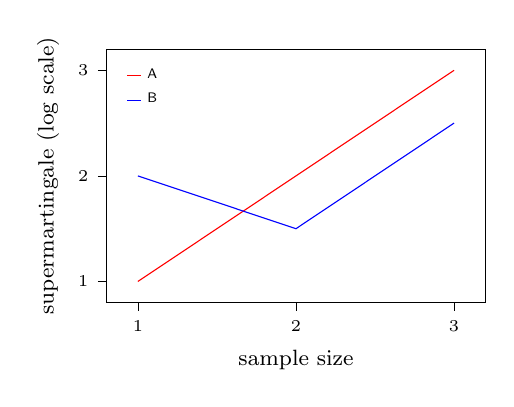
\begin{tikzpicture}
\begin{axis}[
    width=6.4cm,
    height=4.8cm,
    axis lines=box,
    tick align=outside,
    tick style={draw=black, major tick length=3pt},
    xtick pos=bottom, ytick pos=left,
    /pgf/number format/assume math mode=true,
    xlabel={sample size}, ylabel={supermartingale (log scale)},
    label style={font=\fontsize{8}{5}\selectfont},
    tick label style={font=\fontsize{6.4}{4}\selectfont},
    legend pos=north west,
    legend style={
    	font=\sffamily\fontsize{5}{5}\selectfont,
    	draw=none
    	},
    legend image post style={
        xscale=0.3
    }
]


\addplot[color=red] coordinates {(1,1) (2,2) (3,3)};
\addplot[color=blue] coordinates {(1,2) (2,1.5) (3,2.5)};
%\addplot table[x=dof, y=L2] {data.dat};

\legend{A,B}

\end{axis}
\end{tikzpicture}

\end{document}
